\documentclass[a4paper,UTF8]{ctexart}

\usepackage{amsmath, amsthm, amssymb, amsfonts, hyperref, mathrsfs}%美国数学学会的包+?
\usepackage{geometry} %控制界面
\usepackage{bookmark}
\usepackage{fancyhdr} % header & footer
\usepackage{appendix} % 附录
\usepackage{tikz} %作图
\usepackage{graphicx} %插入图片的宏包
\usepackage{float} %设置图片浮动位置的宏包
%\usepackage{subfigure} %插入多图时用子图显示的宏包
\usepackage{listings} %引用代码
\usepackage{physics,mathtools} %物理数学工具
\usepackage{comment}
\usepackage{framed}
\usepackage{caption}
\usepackage{subcaption}
\geometry{top=2.5cm,bottom=2.5cm,left=2.5cm,right=2.5cm} % 布局要求
\pagestyle{fancy} % fancy分格
\fancyhf{} % 清除所有页眉页脚
\renewcommand\headrulewidth{0.6pt}
\renewcommand\footrulewidth{0.6pt}
% font
\setCJKmainfont{Noto Serif CJK SC}[BoldFont={Noto Serif CJK SC Bold}, ItalicFont=]
\lhead{何金铭 PB21020660$\mid$座位号:3}
\cfoot{光的力学效应及光阱PN力的测量预习报告}
\rhead{\thepage}
\lfoot{2024.4.15}
\rfoot{USTC}
%\bibliographystyle{plain} % 引用样式
\everymath{\displaystyle} % display
%============================================================

\begin{document}

\begin{center}
    \textbf{\Large 光的力学效应及光阱PN力的测量预习报告}
    \par \text{\large 何金铭 PB21020660}
\end{center}

\section{实验目的}

光具有能量和动量,光的动量是光的基本属性。携带动量的光与物质相互作用,它们间会有动量的交换,从而表现为光对物体施加一力,作用在物体上的力就等于光引起的单位时间内物体动量的改变。并由此可引起的物体的位移,速度状况的变化,我们称之为光的力学效应。


\section{实验原理}

\subsection{光镊——单光束梯度力光阱}

光作用于物体时,将施加一个力到物体上。由于光辐射对物体产生的力常常表现为压力,因而通常称之为辐射压力或简称光压。然而,在特定的光场分布下,光对物体也可产生一拉力。从而有可能某种特定光场来形成束缚粒子的势阱。

设小球的大小明显大于光波长,可以采用几何光学近似。设小球的折射率$n_1$大于周围媒质的折射率$n_2$。

\begin{figure}[H]
    \centering
    \begin{minipage}[b]{0.9\textwidth}
        \centering
        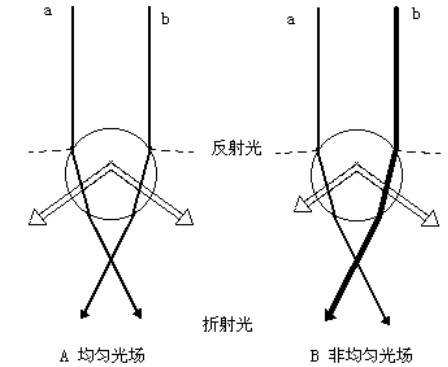
\includegraphics[width=0.6\textwidth]{./fig1.jpg}
        \caption{均匀光场与非均匀光场中的透明小球}
    \end{minipage}
\end{figure}

如果小球处在一个非均匀光场中,如上图B,沿Z方向传播,自左向右光强增大的光场。与左边的光线a相比,
右边较强的光线b作用于小球,使小球获得较大的动量,从而产生较大的力$F_b$。结果总的合力在横向不再平衡,
而是把小球推向右边光强处。小球在这样一个非均匀(即强度分布存在梯度)的光场中所得到的指向光强强的地方的力称之为梯度力($F_g$)

所谓光镊,即单光束梯度力光阱,就是由一束强会聚的激光束构成的。在这样的光场中,粒子
(其折射率$n_1$大于周围煤质的折射率$n_2$)将受到一指向光最强点(焦点)的梯度力。
也就是说光对粒子不仅有推力还可以有拉力。这样,粒子就可能被约束在光最亮点附近。

下图显示了高度会聚的光束锥,经小球折射,将施加一梯度力在小球上。设小球的折射率为n,
液体的折射率为$n_1$,当$n>n_1$时,一对典型的光线a和b经折射后产生力$F_a$和$F_b$,
它们的矢量和是指向焦点f的。实际上,光锥中所有光线施加在小球上的合力F也是指向焦点f的。
当小球的球心O和焦点f间有偏离时,合力F总是使小球趋向焦点。实际上,当光穿过小球时,
在小球表面也产生一定的反射,这将施加一推力于小球,此力常称之为散射力($F_s$)。
只有焦点附近的梯度力大于散射力时才能形成一个三维光学势阱而稳定地捕获微粒。
也就是说,这样的光束可以像镊子一样夹持微粒,移动并操控微粒。

\begin{figure}[H]
    \centering
    \begin{minipage}[b]{0.9\textwidth}
        \centering
        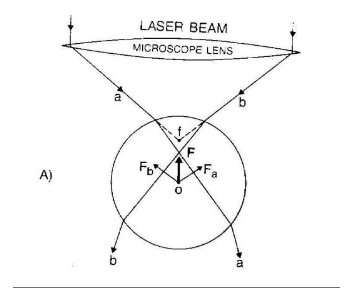
\includegraphics[width=0.6\textwidth]{./fig2.jpg}
        \caption{单光束梯度力光阱原理}
    \end{minipage}
\end{figure}

综上所述,透明微粒在光场中受到的力包括梯度力和散射力($F = F_g + F_s$)。
光阱主要是依靠光梯度力形成的。稳定的捕获是梯度力和散射力平衡的结果。
散射力总是沿光线方向推跑微粒,而梯度力则是把微粒拉向激光的聚焦点处。

\subsection{光阱力测量的流体力学法}

光镊可以捕获和操控微粒,也可以测量作用在微粒上的力。光镊形成的势阱(光阱) 的力学参数在实际应用中十分重要。特别是它的最大捕获力或最大阱力。

光阱力的测量方法大体上有二类:热运动位移法和流体力学法。由于流体力学法具有简单直观的优点,本实验采用了流体力学法。其基本原理如下:

光阱操纵微粒相对流体运动时,微粒将受到液体的粘滞阻力$f$。随着相对速度的增大, 粘滞阻力 $f$ 也随之增大。
当速度超过一定的临界值,粘滞阻力 $f$ 将大于光阱的最大束缚力$F$, 粒子就要从这光阱中逃逸出来。
所以最大阱力${F}_\mathrm{max}$的测量是基于找出光阱操纵微粒所能达到的最大速度 $V_{max}$,
即所谓的逃逸速度。光阱最大阱力 ${F}_\mathrm{max}$的大小就等于这一速度下的粘滞阻力
 $f_{max}$, 但方向相反。在这一速度下的粘滞阻力 $f_{max}$, 可由流体力学中的 Stokes 公式计算:

\begin{equation}
    f_{max}=6\pi \eta r V_{max}
\end{equation}

其中$\eta$为粘滞系数,r 为微粒的半径,$V_{max}$为逃逸速度。

\section{实验内容}

\subsection{实验装置}

图3为本实验所用装置(称之为激光力学参数测量装置)的示意图,包括一个作为光
镊光源的半导体激光器,显微镜,自动样品台,激光器与显微镜的光学耦合光路,以及一套观察和记录光阱对微粒的操作过程的实时监测系统。

\begin{figure}[H]
    \centering
    \begin{minipage}[b]{0.9\textwidth}
        \centering
        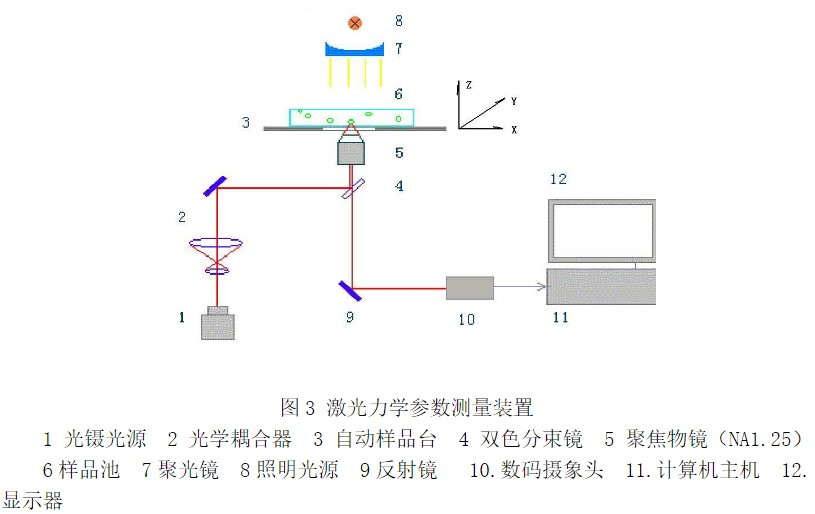
\includegraphics[width=0.9\textwidth]{./fig3.jpg}
    \end{minipage}
\end{figure}

由半导体激光发出的激光束,经过光学耦合光路扩束整形后,入射到双色分束镜上,被反射至物镜聚焦在样品池中形成光阱。捕获和操控过程的观察,类似于普通的显微镜。
照明光通过聚光镜照明样品池,池中的微粒被捕获和操控的图象经物镜后,透过双色分束镜,被反射镜反射到CCD数码摄像头,由显示器显示。也可通过目镜进行观察。数码摄像头获取的信息可以由计算机采集和处理。

实验中所用的样品有很大的挑选余地。只要对所用的激光吸收很小,折射率比周围液体的大,尺度在微米量级就可以。
我们实验中用的是悬浮于液体中的$1-3\mu m$的聚本乙烯小球或$4-5\mu m$的酵母细胞。

\subsection{光陷阱效应}

光陷阱效应表现为当粒子靠近光阱中心,到一定距离时,就受到阱力的作用,被吸引到光阱的中心,也就是说粒子被光阱捕获了。实验中光阱在空间中是固定的,通过移动样品台,使视场中某个微粒接近光阱,观察光阱对粒子的捕获过程。记录粒子被光阱捕获前后的位置,可计算出阱域的大小,即光阱的作用力范围。图4中“十”字叉丝的中心为光镊的阱位(下同)。

\begin{figure}[H]
    \centering
    \begin{minipage}[b]{0.9\textwidth}
        \centering
        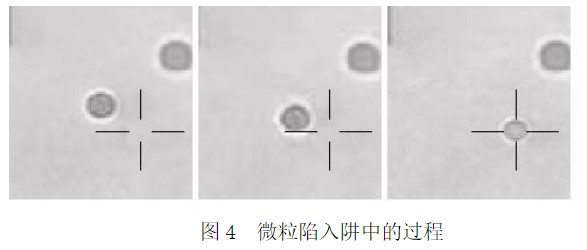
\includegraphics[width=0.9\textwidth]{./fig4.jpg}
    \end{minipage}
\end{figure}

\subsection{光镊在横向(X-Y平面)操控微粒}

如图5所示,光镊已捕获了样品池中的一个粒子。实验中固定光束(即光镊不动),沿X-Y平面移动样品台(池)。这时可以观察到背景的粒子也跟随平台相对光束移动,而被捕获的粒子不动,即实现了光镊操控小球的横向运动。

\begin{figure}[H]
    \centering
    \begin{minipage}[b]{0.9\textwidth}
        \centering
        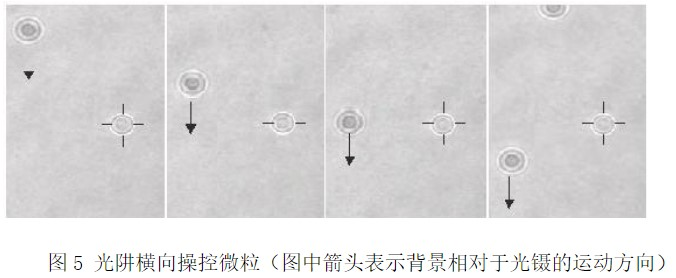
\includegraphics[width=0.9\textwidth]{./fig5.jpg}
    \end{minipage}
\end{figure}

\subsection{光镊在纵向(Z轴方向)操控微粒}

如图6所示,光镊捕获了一微粒。调节物镜与样品台的距离,也即改变了光阱在纵向的位置。这时被捕获的粒子也随之移动,因而它的像依然清晰,而背景中的粒子并不移动,这意味着它们偏离了成像清晰的平面,它们的图像就变得逐渐模糊了(图6b)。这一现象表明光镊实现了对粒子的纵向操控。

\begin{figure}[H]
    \centering
    \begin{minipage}[b]{0.9\textwidth}
        \centering
        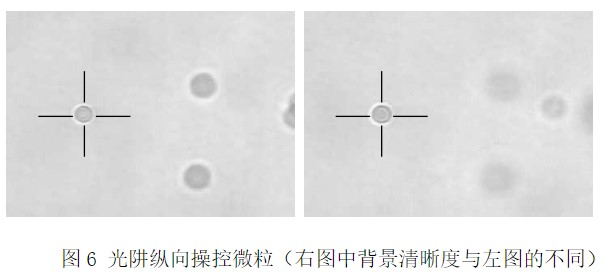
\includegraphics[width=0.9\textwidth]{./fig6.jpg}
    \end{minipage}
\end{figure}

\subsection{光镊最大横向阱力的测量}

在相对静止的液体环境中,用光镊捕获一个微粒,并提升到离样品池底一固定高度处(参考图4),
然后用计算机控制样平台在水平面上产生定向运动(参考图5),运动速度由计算机控制。
刚开始平台以较小速度运动,如果微粒仍在光镊中处于被捕获状态,则逐步加大平台运动速度,重复上述操作。
直到平台速度达到某临界值,微粒从光镊中逃逸出去,此时的平台运动速度即为逃逸速度。
将它代入Stokes公式,即可算得光镊的最大捕获力。粒子在光阱中受到的力与粒子偏离光阱中心的距离有关。
原则上可以测量阱力与位移的关系。位移的测量对实验装置的要求较高,本实验只测量这个最大捕获力。

\end{document}